\section{Durchführung}
\label{sec:Durchführung}

Die wesentlichen Bestandteile des Versuchsaufbaus, der in Abbildung
\ref{fig:aufbau} dargestellt ist, sind eine Cu-Röntgenrühre, ein
LiF-Kristall, sowie ein Geiger-Müller-Zählrohr.
Die Elektronik zur Steuerung ist im Röntgengerät integriert und
wird über einen Computer gesteuert.

\begin{figure}
  \centering
  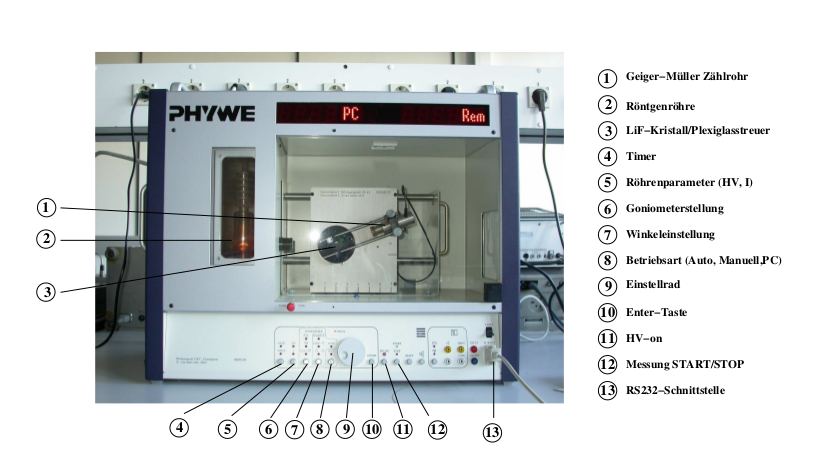
\includegraphics[height=7cm]{aufbau.png}
  \caption{Röntgengerät mit Cu-Röntgenrühre,LiF-Kristall und Geiger-Müller-Zählrohr.}
  \label{fig:aufbau}
\end{figure}

Zu Beginn wird die Bragg-Bedingung überprüft, indem der LiF-Kristall auf einen
festen Kristallwinkel von $\theta=14°$ eingestellt wird und das Geiger-Müller-Zählrohr die
Röntgenstrahlng in einem Bereich von $\alpha_{GM}=26-30°$ misst.\\

Anschließend wird das Emissionsspektrum der Cu-Röntgenröhre untersucht, indem
der 2:1 Koppelmodus eingestellt wird und das Röntgenspecktrum im Bereich von
$\alpha_{GM}=4-26°$ gemessen wird.\\

Nun wird das Absorptionsspektrum für fünf verschiedener Materialen untersucht.
Dazu wird ein abgeschätzter Bereich um den zuvor berechneten gemessen.
Für diese Messung wurden Brom, Zink, Strontium, Aluminium und Gold ausgewählt.\\
